\begin{Problem}{ICPC}{\divsel{1}{3}}

ICPC国际大学生程序设计竞赛是全球最具影响力的大学生程序设计竞赛。比赛以团队的形式进行,需要在5个小时内解决至多13道题目。程序完成之后提交裁判运行,运行的结果会判定为正确或错误并及时通知参赛队。有趣的是,每队在正确解答一题后,组织者将在其位置上升起一只代表该题颜色的气球,每道题目第一支解决掉它的队还会额外获得一个“FIRST PROBLEM SOLVED”的气球,也就是所谓的“一血气球”。

\begin{figure}[h]
\centering
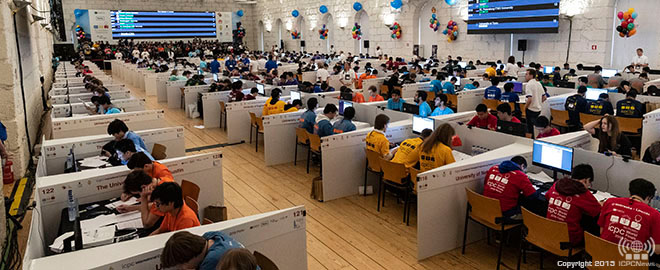
\includegraphics[width=12cm]{src/scoreboard/porto.jpg}
\caption{ICPC 2019 World Finals}
\end{figure}

ICPC最后的获胜者为正确解答题目最多且总用时最少的队伍。每道试题用时将从竞赛开始到试题解答被判定为正确为止,其间每一次提交运行结果被判错误的话将被加罚20分钟时间,未正确解答的试题不记时。

JYY在参加完一场ICPC竞赛后,观察了最终的榜单,他想知道自己在比赛中的策略是否可以改进。确切的说,JYY想知道,如果在比赛中他改变了做题的顺序,最多能够拿到多少个“一血气球”,以及拿到的最好名次是多少。

在本题中,为了简化问题,我们不考虑罚时,并且假定:
\begin{itemize}
\item JYY所在队伍完成第一道题(即完成时间最早的那题)所需花费的时间即为通过该题时刻,此后完成每道题所需花费的时间为通过该题的时刻减去通过上一题的时刻;
\item JYY改变做题顺序不会影响解答每道题所花费的时间;
\item JYY所在队伍在比赛中没有做出来的题,改变做题顺序后仍然做不出来;
\item 若存在多支队伍在同一个最小时刻解决某道问题,则这些队伍都能获得“一血气球”。
\end{itemize}

最终所有队伍先按照正确解答的题目数量从大到小排名,正确解题数相同的队伍,按照总用时从小到大排名。总用时是指通过每道题的时刻之和。若存在多支队伍过题数,罚时均相同,则这些队伍获得相同的、较优的排名。例如,第一支队通过了7题,总用时100分钟,第二支队通过了7题,总用时100分钟,第三支队通过了6题,总用时70分钟,则在这三支队中,第一、第二支队并列第一名,第三支队是第三名。

\subsection*{输入格式}

输入的第一行包含两个整数$n, m$ $(2 \leq n \leq 1000, 1 \leq m \leq \divsel{13}{10})$,表示参加比赛的团队数量和这场比赛中题目的数量。

接下来$n$行,每行包含$m$个整数,表示一支队伍的通过每道题的时刻(单位:分钟)。具体来说,第$i$行的第$j$个整数$a_{ij}$ $(0 < a_{ij} < 300)$ 表示第$i$只队伍通过第$j$道题的时间。如果第$i$支队没有通过第$j$题,$a_{ij}$将会以\texttt{-}代替。保证对于每个队,在同一分钟内最多通过一题。

JYY所在的队伍是第一支队。

\subsection*{输出格式}

输出一行包括两个整数,即最多能够拿到多少个“一血气球”和最高能取得的名次。为实现这两个目标,你可以分别采取两种不同的做题顺序。

\exmpv{01-sample}
\exmpv{02-sample}

\end{Problem}

